\documentclass[10pt]{article}
\usepackage[margin=0.78in]{geometry}
\usepackage[T1]{fontenc}
\usepackage{lmodern,microtype,booktabs,graphicx,xcolor,hyperref,placeins}
\definecolor{navy}{HTML}{16324F}\definecolor{teal}{HTML}{087E8B}
\hypersetup{colorlinks=true,linkcolor=navy,urlcolor=teal}
\title{\textcolor{navy}{When Should IDM-Viz Request Labels?}\\[3pt]
\large Delayed Audit Policies Under Explicit Acquisition Budgets}
\author{23I-2581 and 23I-2604\\Data Analysis and Visualization --- Phase 3 addendum}
\date{17 November 2026}
\begin{document}\maketitle
\begin{abstract}
We replay six predeclared audit policies on cached predictions from the 30-seed locked synthetic evaluation. The matrix crosses four label delays (0, 5, 20, 100 batches), three audit budgets (2, 4, 8 cohorts), and strict-cap versus exact-quota spending. It evaluates whether selected audits identify harmful batches and whether harmful episodes can be verified before the 24-batch horizon ends. The replay is outcome-informed for evaluation and is not fresh independent confirmation.
\end{abstract}
\section{Protocol and label timing}
Input-alarm and calibrated-concern thresholds are quantiles set only on five disjoint development seeds at a rate of $B/24$, where $B$ is the cohort budget. The conjunction requires both signals; the disjunction accepts either signal or a previously released error signal. The released-error policy starts with a fixed probe at $\lceil24/B\rceil$, then compares the historical reference accuracy with selected-label accuracy once labels are available. Uniform selection spaces acquisitions across the horizon. Every selected cohort contains 500 rows.

At decision clock $t$, a selected source cohort $s$ is usable only if $s+d<t$. Thus its first usable clock is $s+d+1$. The strict-cap mode acquires only on a positive policy signal and may leave budget unused. Exact-quota mode fills any remaining quota in the tail; those forced acquisitions are separately counted and must not be interpreted as signal-driven evidence. A harmful cohort is defined as evaluator accuracy strictly more than 0.05 below the frozen historical reference. Episodes are maximal contiguous runs of such cohorts.

The 30 evaluation seeds are paired across all policies. The run-level receipt includes within-condition paired intervals. This report additionally averages each seed over matched conditions and budgets before bootstrapping the 30 seed-level differences against uniform. Batches, budgets, and conditions are not treated as independent replicates. Conditions are not independent real-world domains.
\section{Results}
\begin{figure}[ht]
\centering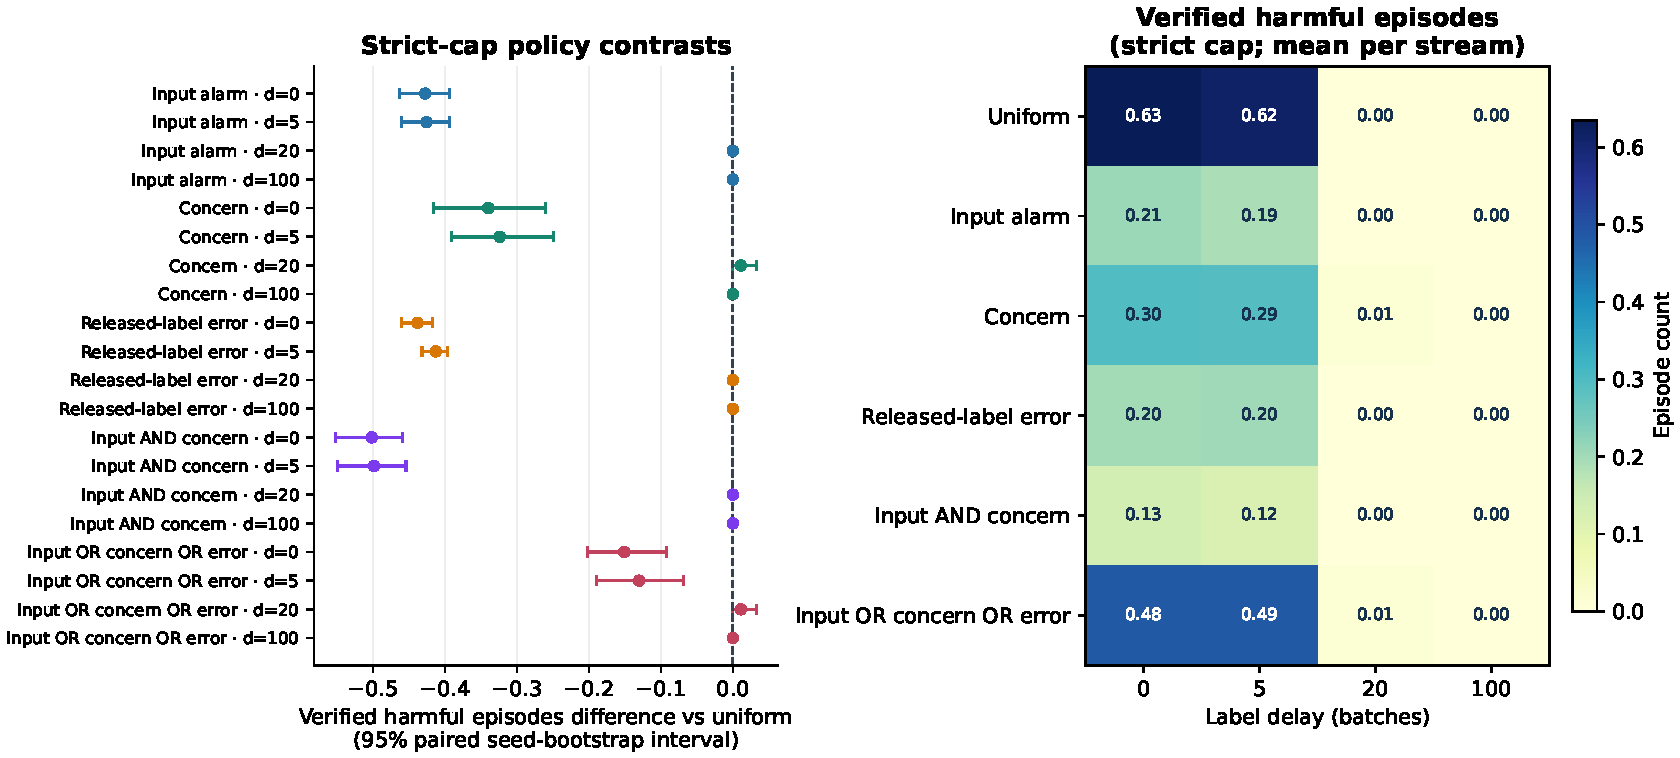
\includegraphics[width=\linewidth]{audit_policy_effects.pdf}
\caption{Left: strict-cap paired differences versus uniform in harmful episodes verified by stream end, averaged within seed across matched conditions and budgets; intervals are 95\% seed-bootstrap intervals. Right: strict-cap verification yield by policy and delay, averaged across budgets, conditions, and seeds. A delay of 100 exceeds the simulated stream horizon, so no selected label can be verified online within that horizon.}
\end{figure}
\begin{table}[ht]
\centering\small\begin{tabular}{@{}lrrr@{}}\toprule
Policy & Strict audits & Strict unused & Exact forced\\\midrule
Uniform & 4.67 & 0.00 & 0.00 \\
Input alarm & 2.33 & 2.33 & 2.33 \\
Concern & 1.88 & 2.79 & 2.79 \\
Released-label error & 1.11 & 3.56 & 3.24 \\
Input AND concern & 0.71 & 3.96 & 3.96 \\
Input OR concern OR error & 3.87 & 0.80 & 0.76 \\\bottomrule\end{tabular}
\caption{Average acquisition use across seeds, conditions, delays, and budgets. Exact-quota counts show tail acquisitions not triggered by a policy signal.}
\end{table}
\FloatBarrier
\section{Interpretation}
The matrix separates two questions that the earlier fixed-quota comparison conflated: whether a policy chooses informative audits under a hard cost cap, and what happens when an operator insists on spending the full quota. Strict-cap contrasts are not matched by acquisition volume: uniform uses a mean 4.67 cohorts, while signal policies range from 0.71 (conjunction) to 3.87 (disjunction). Their lower verified-episode counts therefore mix policy selectivity with fewer audit opportunities and do not establish inferior ranking at equal spend. Exact-quota performance includes the forced tail acquisitions shown in Table 1, so it is a budget-completion scenario rather than a pure alarm policy. Longer delays reduce opportunities to verify episodes, while delay 100 makes online verification impossible over this finite horizon by design.

All metrics involving harmful labels use evaluator truth after decisions are simulated. The released-error arm only consumes selected labels after the release clock condition. This replay cannot show analyst utility, monetary savings, or downstream intervention benefit. Results depend on this synthetic stream, frozen reference, 0.05 harm margin, threshold quantiles, and horizon; no claim of superiority on natural drift is supported.
\section{Reproduction}
From the project root:
\begin{verbatim}
python scripts/run_audit_policy_matrix.py
python scripts/report_audit_policy_matrix.py
tectonic -X compile \\
  reports/phase3/audit_policy_matrix_20261117_v6/audit_policy_matrix.tex
\end{verbatim}
The run lock records all source and output hashes, policy rules, seed banks, thresholds, and limitations. The complete per-seed data, sequential decisions, and paired bootstrap intervals are included alongside this report.
\end{document}
